\documentclass{beamer}
\usepackage{graphicx}
\usepackage{listings}

\usetheme{Madrid}
\usecolortheme{beaver}
\date[26 September 2025]{}

\title{Unconventional reinforcement learning on traffic lights with SUMO}
\subtitle{Master Degree in Computer Science}
% \author{Refolli~F.~865955}
\author[RF 865955]{Francesco~Refolli\\[10mm]{\small Supervisor: Prof. Giuseppe Vizzari}}
\logo{
\includegraphics[height=2.5cm]{logo_unimib.pdf}}

\newcommand{\putimage}[2] {
  \begin{figure}[H]
    \centering
    \includegraphics[width=#2\linewidth]{#1}
	\end{figure}
}

\newcommand{\putimagecouple}[4] {
  \begin{figure}[!htb]
    \centering
    \begin{minipage}{0.45\linewidth}
      \centering
      \includegraphics[width=\linewidth]{#1}
      \caption{#2}
    \end{minipage}
    \hspace{0.25cm}
    \begin{minipage}{0.45\linewidth}
      \centering
      \includegraphics[width=\linewidth]{#3}
      \caption{#4}
    \end{minipage}
  \end{figure}
}

% \begin{frame}
% \frametitle{Outline}
% \tableofcontents
% \end{frame}

\begin{document}

\frame{\titlepage}

\setbeamertemplate{logo}{}

\begin{frame}
  \begin{columns}
    \begin{column}{0.4\textwidth}
      \begin{figure}
        \centering
        
\includegraphics[width=1.0\textwidth]{figures/sumo-logo.png}
      \end{figure}
      \begin{itemize}
        \item Free and Open Source microscopic traffic simulator
        \item Developed at German Aerospace Center (DLR)
        \item Multimodal: cars, trams, bikes, pedestrians ...
        \item Highly customizable
      \end{itemize}
    \end{column}
    \begin{column}{0.6\textwidth}
      \begin{figure}
        \centering
        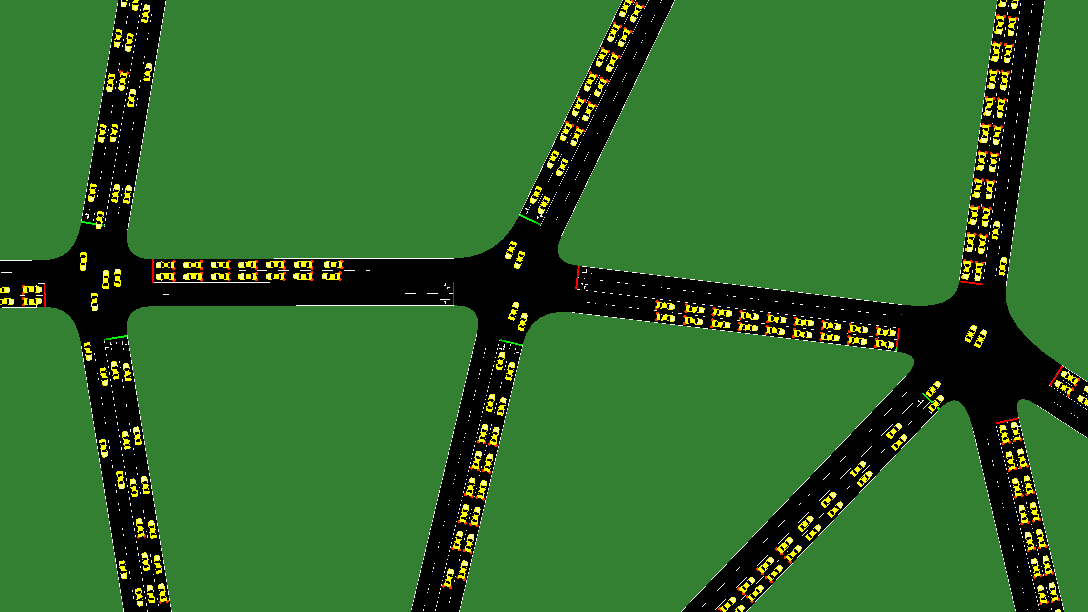
\includegraphics[width=1.0\textwidth]{figures/sumo-example.png}
      \end{figure}
      \begin{figure}
        \centering
        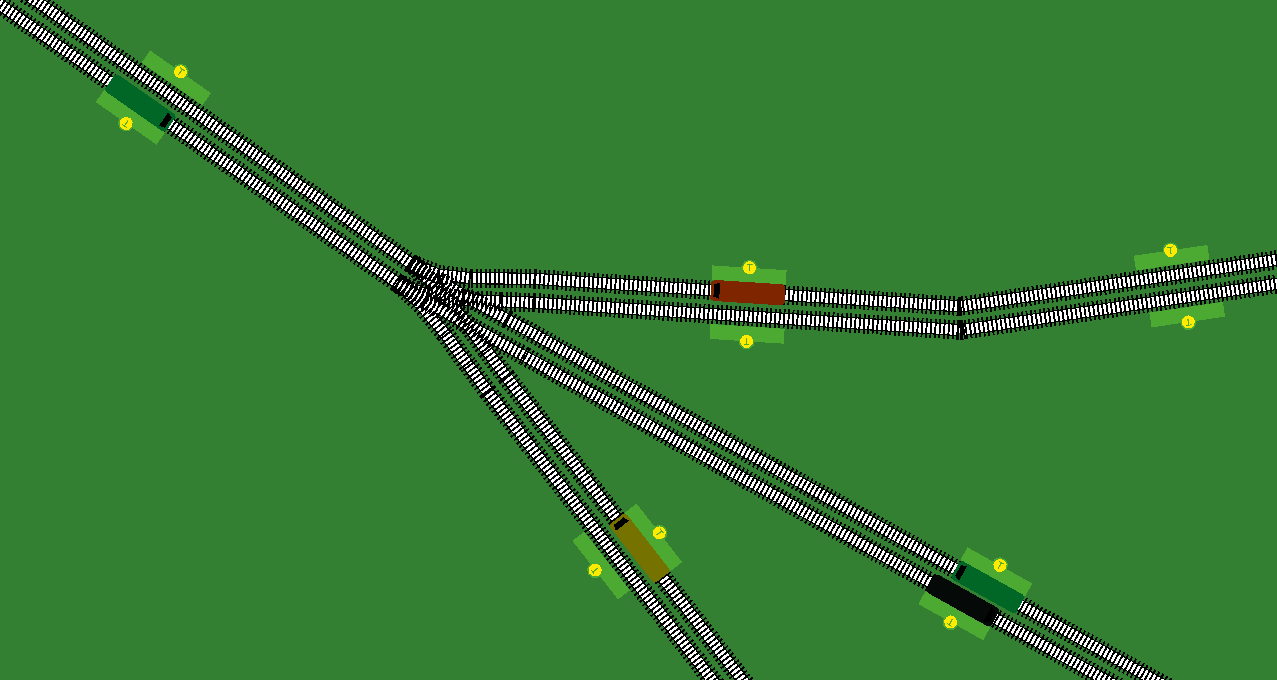
\includegraphics[width=1.0\textwidth]{figures/sumo-example2.png}
      \end{figure}
    \end{column}
  \end{columns}
\end{frame}

\begin{frame}
\frametitle{SUMO-RF: SUMO + Reinforcement Learning}
  A FOSS framework for Reinforcement Learning with SUMO developed as fork of \textit{LucasAlegre/sumo-rl} with a focus on modularity, flexibility and Multi Agent Learning.
  It also contains several utilities for format conversions, metrics analysis and plot, schematic-based demand generation and more.
  \begin{figure}
    \centering
    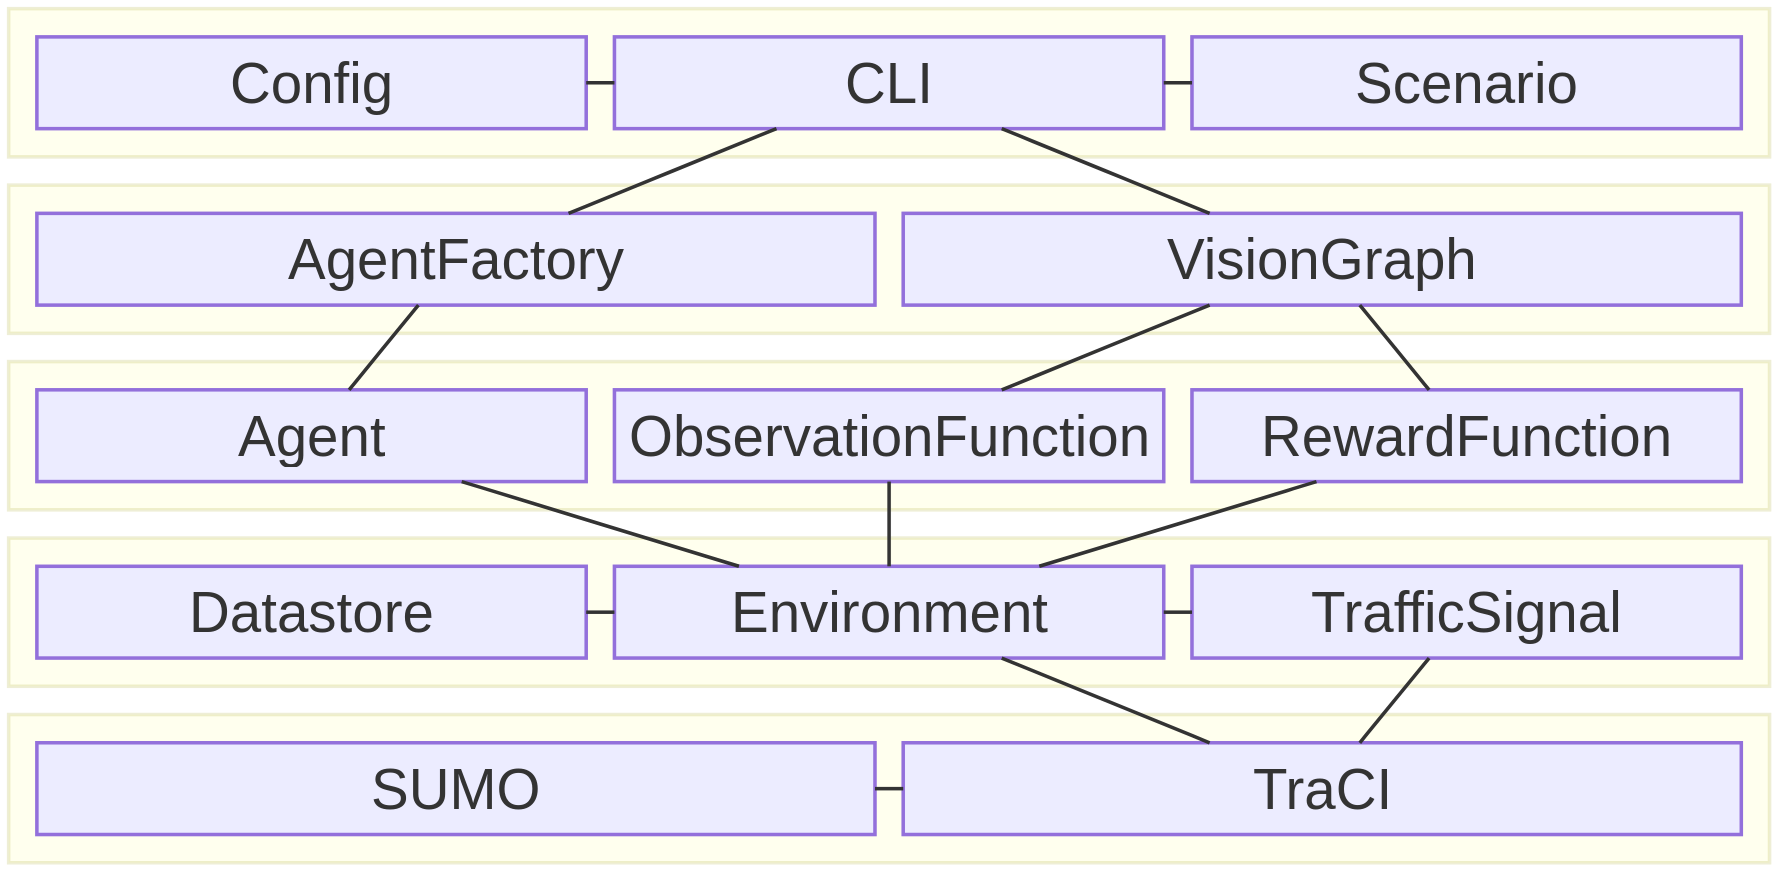
\includegraphics[width=0.8\textwidth]{figures/sumo-rf-architecture.png}
  \end{figure}
\end{frame}

\begin{frame}
\frametitle{The Agent Model}
\end{frame}

\begin{frame}
\frametitle{The Observation Function}
\end{frame}

\begin{frame}
\frametitle{The Reward Function}
\end{frame}

\begin{frame}
\frametitle{The Action Space}
\end{frame}

\begin{frame}[fragile]
\frametitle{The Dataset}
  \begin{small}
    \begin{verbatim}
    TOK = (£|\*|~|%(,[0-9.]+)?(,[0-9.]+)?|[A-Z][A-Z0-9]+)
    EXP = ^([0-9]+,)?([0-9]+,)?TOK(,TOK)*$
    \end{verbatim}
  \end{small}
\end{frame}

\begin{frame}
\centering
\Huge
Thank You
\end{frame}

\end{document}
